\ifthenelse{\boolean{newnameindexdrawings}}{

\begin{figure}[p]
\bb
\figurepart{1}{2}
\begin{center}
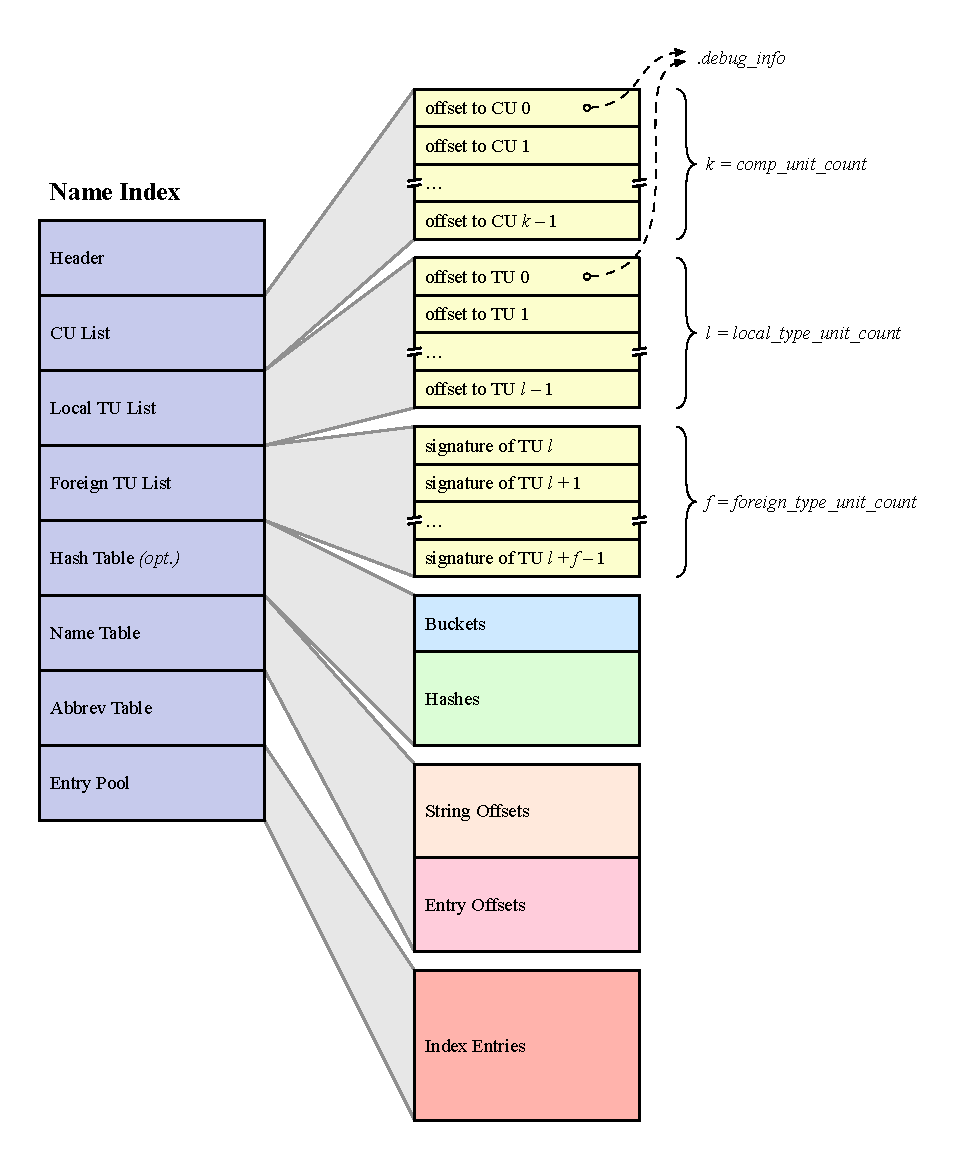
\includegraphics[keepaspectratio=true,scale=1.0]{name-index-drawings-6p1}
\caption{Name Index Layout}
\label{fig:nameindexlayoutpart1}
\end{center}
\eb
\end{figure}
\begin{figure}[p]
\bb
\figurepart{2}{2}
\begin{center}
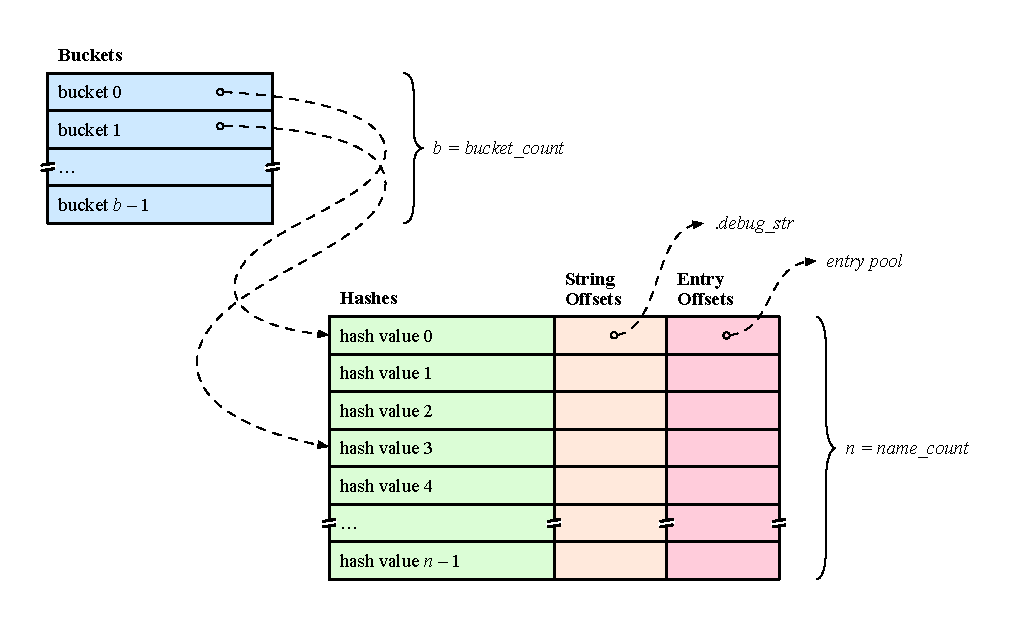
\includegraphics[keepaspectratio=true,scale=1.0]{name-index-drawings-6p2}
%\vspace*{1cm} doesn't put space between the two includes--the space shows
%up after the second inclusion, before the caption.
%The following is a hokey way to fake it, but it works...
  \begin{tikzpicture}
  \draw node (vspace) at (0,0) {\textcolor{white}{vspace}} ;
  \end{tikzpicture}
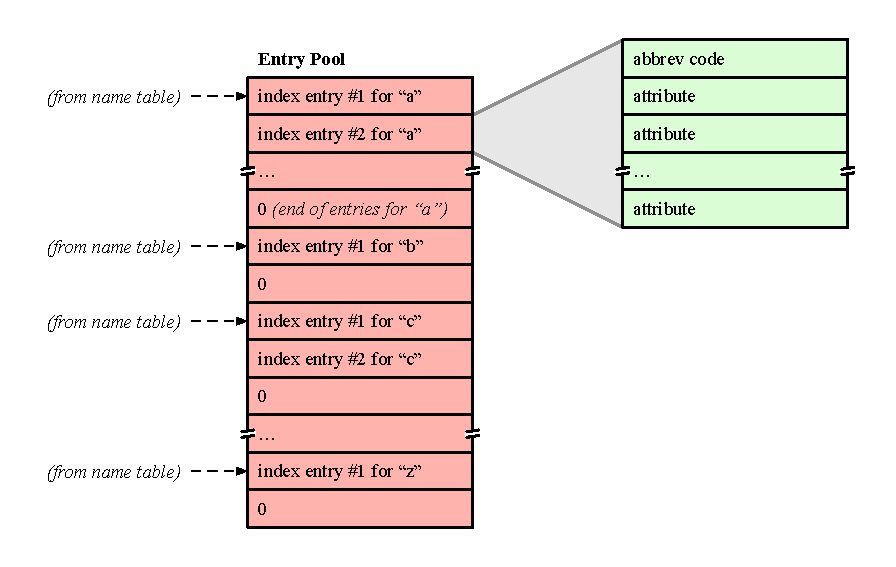
\includegraphics[keepaspectratio=true,scale=1.0]{name-index-drawings-6p3}
\vspace{3mm}
%\caption{Name Index Layout \textit{(concluded)}}
Figure~\ref{fig:nameindexlayoutpart1}: Name Index Layout \textit{(concluded)}
%\label{fig:nameindexlayoutpart2}
\end{center}
\eb
\end{figure}

} % end new name table figure
{ % begin earlier name table figure

\begin{figure}[p]
\begin{center}
\newcommand{\thistypesize}{\footnotesize}
\newcommand{\thisblue}{blue!10}
\newcommand{\thisyellow}{yellow!20}
% \invispblu and \invispyel are used to insert an invisible letter
% with a descender in lines that otherwise do not have one. This
% makes the spacing and bounding box dimensions more uniform.
\newcommand{\invispblu}{\textcolor{\thisblue}{p}}
\newcommand{\invispyel}{\textcolor{\thisyellow}{p}}
  \begin{tikzpicture}[
        every node/.style={draw, anchor=text,
          node distance=2.5cm,
          text width=3.5cm, font=\thistypesize},
        description/.style={
          draw=none,
          font=\em\thistypesize,
          node distance=5cm,
          text width=5cm
        },
        table/.style={
          font=\thistypesize,
          draw=black,
          rectangle split,
          fill=\thisyellow
        },
        caption/.style={
          anchor=south,
          font=\thistypesize,
          draw=none
        }]
    \node (header) [font=\thistypesize,
                    fill=\thisblue,
                    rectangle split,
                    rectangle split allocate boxes=8,
                    rectangle split parts=8] at (0, -1)
          {Header\invispblu
            \nodepart{two}
            CU list\invispblu
            \nodepart{three}
            Local TU list\invispblu
            \nodepart{four}
            Foreign TU list\invispblu
            \nodepart{five}
            Hash table\invispblu
            \nodepart{six}
            Name table\invispblu
            \nodepart{seven}
            Abbrev table\invispblu
            \nodepart{eight}
            Entry pool\invispblu
          };
    \draw node [caption] at (header.north) {Name Index} ;

    \node (cuofs) [table,
                   rectangle split allocate boxes=4,
                   rectangle split parts=4]  at (8,0)
         {CU 0 offset\invispyel
          \nodepart{two}
          CU 1 offset\invispyel
          \nodepart{three}
          \dots
          \nodepart{four}
          CU $c-1$ offset\invispyel
         };
        \node (cusecofs) [description,right of=cuofs] {section offset \\ of CU header} ;
        
    \node (tuofs) [below of=cuofs,
                   table,
                   rectangle split allocate boxes=4,
                   rectangle split parts=4]
         {TU 0 offset\invispyel
          \nodepart{two}
          TU 1 offset\invispyel
          \nodepart{three}
          \dots
          \nodepart{four}
          TU $t-1$ offset\invispyel
         };
        \node (tusecofs) [description,right of=tuofs] {section offset \\ of TU header} ;
        
    \node (tusigs) [below of=tuofs, 
                    table,
                    rectangle split allocate boxes=4,
                    rectangle split parts=4]
         {TU $t$ signature\invispyel
          \nodepart{two}
          TU $t+1$ signature\invispyel
          \nodepart{three}
          \dots
          \nodepart{four}
          TU $t+f-1$ signature\invispyel
         };
   \node (typesigs) [description,right of=tusigs] {type signature \\ of foreign TU} ;

   \matrix (hashtable) [draw,style=dashed,column sep=8mm] at (1, -9)
           {\node (buckets) [style=solid, table, text width=3cm,
                             rectangle split allocate boxes=4,
                             rectangle split parts=4]
                  {               hash index 0\invispyel
                  \nodepart{two}  hash index 1\invispyel
                  \nodepart{three}\dots
                  \nodepart{four} hash index $b-1$\invispyel
                  } ;
            \draw node [caption] at (buckets.north) {~Buckets} ;
            &
            \node (hashes) [style=solid, table, text width=3cm,
                            rectangle split allocate boxes=6,
                            rectangle split parts=6]
                  {               hash value 0\invispyel
                  \nodepart{two}  hash value 1\invispyel
                  \nodepart{three}hash value 2\invispyel
                  \nodepart{four} hash value 3\invispyel
                  \nodepart{five} \dots
                  \nodepart{six}  hash value $n-1$\invispyel
                  } ;
            \draw node [caption] at (hashes.north) {~Hashes} ;
            \\
           };
    \node (names) [right of=hashes, node distance=5cm,
                   style=solid,
                   table,
                   text width=4cm,
                   rectangle split allocate boxes=6,
                   rectangle split parts=6]
          {                name 0\hspace{9mm} entry 0
           \nodepart{two}  name 1\hspace{9mm} entry 1\invispyel
           \nodepart{three}name 2\hspace{9mm} entry 2\invispyel
           \nodepart{four} name 3\hspace{9mm} entry 3\invispyel
           \nodepart{five} \dots
           \nodepart{six}  name $n-1$\hspace{2.7mm} entry $n-1$\invispyel
          };
    \draw node [caption] at (names.north) {\hspace*{-2mm}Strings\hspace*{10mm}Entries} ;
    \path (names.north) edge (names.south) ;
         
    \node (entries) [below of=hashtable, node distance=6cm, xshift=-2cm, yshift=-5mm,
                   style=solid,
                   table,
                   rectangle split allocate boxes=12,
                   rectangle split parts=12]
           {                  index entry \#1 for "a"
            \nodepart{two}    index entry \#2 for "a"
            \nodepart{three}  ...
            \nodepart{four}   0
            \nodepart{five}   index entry \#1 for "b"
            \nodepart{six}    0
            \nodepart{seven}  index entry \#1 for "c"
            \nodepart{eight}  index entry \#1 for "c"
            \nodepart{nine}   0
            \nodepart{ten}    ...
            \nodepart{eleven} index entry \#1 for "z"
            \nodepart{twelve} 0
           };
    \draw node [caption] at (entries.north) {Index entries} ;
    
    \node (entry) [right of=entries, xshift=4cm, yshift=2cm,
                   style=solid,
                   table,
                   rectangle split allocate boxes=5,
                   rectangle split parts=5]
           {                 abbrev code
            \nodepart{two}   attribute
            \nodepart{three} attribute
            \nodepart{four}  ...
            \nodepart{five}  attribute
           };
    \draw node [caption] at (entry.north) {Index Entry} ;

    \draw[thick, double distance=3pt, implies-space] (header.two east)   -- (cuofs.west) ;
    \draw[thick, double distance=3pt, implies-space] (header.three east) -- (tuofs.west) ;
    \draw[thick, double distance=3pt, implies-space] (header.four east)  -- (tusigs.west) ;
    \draw[thick, double distance=3pt, implies-space] (entries.one east)  -- (entry.west) ;
    
    \path[-triangle 45]
        (cuofs)              edge (cusecofs)
        (tuofs)              edge (tusecofs)
        (tusigs)             edge (typesigs)
        (buckets.one east)   edge (hashes.one west)
        (buckets.two east)   edge (hashes.three west)
        (buckets.three east) edge (hashes.six west)
        ;
    \path[loosely dashed, thin, open triangle 45-open triangle 45]
        (hashes.one east)    edge (names.one west)
        (hashes.two east)    edge (names.two west)
        (hashes.three east)  edge (names.three west)
        (hashes.four east)   edge (names.four west)
        (hashes.five east)   edge (names.five west)
        (hashes.six east)    edge (names.six west)
        ;
    \draw[thick, double distance=3pt, implies-space] (header.five east) 
        .. controls +(south east:2cm) .. (hashtable.north) ;
    \draw[thick, double distance=3pt, implies-space] (header.six east)
        .. controls (hashes.north west) and (tusigs.south east) .. (names.north) ;
    \draw[thick, double distance=3pt, implies-space] (header.south) 
        .. controls (-1,-8)  and (-1, -14) .. (entries.west) ;

    \node [text width=8cm, draw=none] at (6,-17.5) {\textit{Notes:}} ;   
    \draw [thick, double distance=3pt, implies- ] (6,-18) -- (7.3,-18)
          node[right=2mm, text width=9cm, draw=none, node distance=1cm] 
          {\textit{indicates an expanded view of the indicated part}} ;
    \draw [loosely dashed, thin, open triangle 45-open triangle 45] (6,-18.5) -- (7.3,-18.5) 
          node[right=2mm, text width=9cm, draw=none] {\textit{indicates correspondence}} ;
    \node [text width=11cm, draw=none] at (6,-19)
          {\textit{Where  n=name\_count, b=bucket\_count, c=comp\_unit\_count, 
          f=foreign\_type\_unit\_count, t=local\_type\_unit\_count}} ;
              
  \end{tikzpicture}

\end{center}
\caption{Name Index Layout}
\label{fig:nameindexlayout}
\end{figure}

} % end old name table figure
